\documentclass[twoside]{book}

% Packages required by doxygen
\usepackage{fixltx2e}
\usepackage{calc}
\usepackage{doxygen}
\usepackage{graphicx}
\usepackage[utf8]{inputenc}
\usepackage{makeidx}
\usepackage{multicol}
\usepackage{multirow}
\PassOptionsToPackage{warn}{textcomp}
\usepackage{textcomp}
\usepackage[nointegrals]{wasysym}
\usepackage[table]{xcolor}

% Font selection
\usepackage[T1]{fontenc}
\usepackage{mathptmx}
\usepackage[scaled=.90]{helvet}
\usepackage{courier}
\usepackage{amssymb}
\usepackage{sectsty}
\renewcommand{\familydefault}{\sfdefault}
\allsectionsfont{%
  \fontseries{bc}\selectfont%
  \color{darkgray}%
}
\renewcommand{\DoxyLabelFont}{%
  \fontseries{bc}\selectfont%
  \color{darkgray}%
}
\newcommand{\+}{\discretionary{\mbox{\scriptsize$\hookleftarrow$}}{}{}}

% Page & text layout
\usepackage{geometry}
\geometry{%
  a4paper,%
  top=2.5cm,%
  bottom=2.5cm,%
  left=2.5cm,%
  right=2.5cm%
}
\tolerance=750
\hfuzz=15pt
\hbadness=750
\setlength{\emergencystretch}{15pt}
\setlength{\parindent}{0cm}
\setlength{\parskip}{0.2cm}
\makeatletter
\renewcommand{\paragraph}{%
  \@startsection{paragraph}{4}{0ex}{-1.0ex}{1.0ex}{%
    \normalfont\normalsize\bfseries\SS@parafont%
  }%
}
\renewcommand{\subparagraph}{%
  \@startsection{subparagraph}{5}{0ex}{-1.0ex}{1.0ex}{%
    \normalfont\normalsize\bfseries\SS@subparafont%
  }%
}
\makeatother

% Headers & footers
\usepackage{fancyhdr}
\pagestyle{fancyplain}
\fancyhead[LE]{\fancyplain{}{\bfseries\thepage}}
\fancyhead[CE]{\fancyplain{}{}}
\fancyhead[RE]{\fancyplain{}{\bfseries\leftmark}}
\fancyhead[LO]{\fancyplain{}{\bfseries\rightmark}}
\fancyhead[CO]{\fancyplain{}{}}
\fancyhead[RO]{\fancyplain{}{\bfseries\thepage}}
\fancyfoot[LE]{\fancyplain{}{}}
\fancyfoot[CE]{\fancyplain{}{}}
\fancyfoot[RE]{\fancyplain{}{\bfseries\scriptsize Generated on Tue Sep 27 2016 22\+:22\+:51 for Lab3 by Doxygen }}
\fancyfoot[LO]{\fancyplain{}{\bfseries\scriptsize Generated on Tue Sep 27 2016 22\+:22\+:51 for Lab3 by Doxygen }}
\fancyfoot[CO]{\fancyplain{}{}}
\fancyfoot[RO]{\fancyplain{}{}}
\renewcommand{\footrulewidth}{0.4pt}
\renewcommand{\chaptermark}[1]{%
  \markboth{#1}{}%
}
\renewcommand{\sectionmark}[1]{%
  \markright{\thesection\ #1}%
}

% Indices & bibliography
\usepackage{natbib}
\usepackage[titles]{tocloft}
\setcounter{tocdepth}{3}
\setcounter{secnumdepth}{5}
\makeindex

% Hyperlinks (required, but should be loaded last)
\usepackage{ifpdf}
\ifpdf
  \usepackage[pdftex,pagebackref=true]{hyperref}
\else
  \usepackage[ps2pdf,pagebackref=true]{hyperref}
\fi
\hypersetup{%
  colorlinks=true,%
  linkcolor=blue,%
  citecolor=blue,%
  unicode%
}

% Custom commands
\newcommand{\clearemptydoublepage}{%
  \newpage{\pagestyle{empty}\cleardoublepage}%
}


%===== C O N T E N T S =====

\begin{document}

% Titlepage & ToC
\hypersetup{pageanchor=false,
             bookmarks=true,
             bookmarksnumbered=true,
             pdfencoding=unicode
            }
\pagenumbering{roman}
\begin{titlepage}
\vspace*{7cm}
\begin{center}%
{\Large Lab3 \\[1ex]\large 1.\+0 }\\
\vspace*{1cm}
{\large Generated by Doxygen 1.8.8}\\
\vspace*{0.5cm}
{\small Tue Sep 27 2016 22:22:51}\\
\end{center}
\end{titlepage}
\clearemptydoublepage
\tableofcontents
\clearemptydoublepage
\pagenumbering{arabic}
\hypersetup{pageanchor=true}

%--- Begin generated contents ---
\chapter{Programación genérica en C++}
\label{index}\hypertarget{index}{}\begin{DoxyAuthor}{Author}
Dunia Barahona \href{mailto:s4si@hotmail.com}{\tt s4si@hotmail.\+com} 
\end{DoxyAuthor}
\begin{DoxyDate}{Date}
11 de setiembre de 2016 
\end{DoxyDate}
\begin{DoxyVersion}{Version}
1.\+0 
\end{DoxyVersion}
\begin{DoxyParagraph}{Descripción}
Serie de clases que modelan figuras geométricas. La clase base se llama \hyperlink{class_figura}{Figura} y las derivadas son \hyperlink{class_circulo}{Circulo}, \hyperlink{class_cuadrado}{Cuadrado} y \hyperlink{class_triangulo}{Triangulo}; cada una tiene su respectivo archivo de encabezados. Todas estas clases estan implementadas en el \hyperlink{main_8cpp_a3c04138a5bfe5d72780bb7e82a18e627}{main} . 
\end{DoxyParagraph}

\chapter{Class Index}
\section{Class List}
Here are the classes, structs, unions and interfaces with brief descriptions\+:\begin{DoxyCompactList}
\item\contentsline{section}{\hyperlink{class_calculadora}{Calculadora$<$ data $>$} }{\pageref{class_calculadora}}{}
\item\contentsline{section}{\hyperlink{class_fraccion}{Fraccion} }{\pageref{class_fraccion}}{}
\item\contentsline{section}{\hyperlink{class_matriz}{Matriz} }{\pageref{class_matriz}}{}
\item\contentsline{section}{\hyperlink{class_polinomio}{Polinomio} }{\pageref{class_polinomio}}{}
\end{DoxyCompactList}

\chapter{File Index}
\section{File List}
Here is a list of all files with brief descriptions\+:\begin{DoxyCompactList}
\item\contentsline{section}{\hyperlink{_circulo_8cpp}{Circulo.\+cpp} }{\pageref{_circulo_8cpp}}{}
\item\contentsline{section}{\hyperlink{_circulo_8h}{Circulo.\+h} }{\pageref{_circulo_8h}}{}
\item\contentsline{section}{\hyperlink{_cuadrado_8cpp}{Cuadrado.\+cpp} }{\pageref{_cuadrado_8cpp}}{}
\item\contentsline{section}{\hyperlink{_cuadrado_8h}{Cuadrado.\+h} }{\pageref{_cuadrado_8h}}{}
\item\contentsline{section}{\hyperlink{_figura_8cpp}{Figura.\+cpp} }{\pageref{_figura_8cpp}}{}
\item\contentsline{section}{\hyperlink{_figura_8h}{Figura.\+h} }{\pageref{_figura_8h}}{}
\item\contentsline{section}{\hyperlink{main_8cpp}{main.\+cpp} }{\pageref{main_8cpp}}{}
\item\contentsline{section}{\hyperlink{_triangulo_8cpp}{Triangulo.\+cpp} }{\pageref{_triangulo_8cpp}}{}
\item\contentsline{section}{\hyperlink{_triangulo_8h}{Triangulo.\+h} }{\pageref{_triangulo_8h}}{}
\end{DoxyCompactList}

\chapter{Class Documentation}
\hypertarget{class_calculadora}{\section{Calculadora$<$ data $>$ Class Template Reference}
\label{class_calculadora}\index{Calculadora$<$ data $>$@{Calculadora$<$ data $>$}}
}


{\ttfamily \#include $<$Calculadora.\+h$>$}

\subsection*{Public Member Functions}
\begin{DoxyCompactItemize}
\item 
\hyperlink{class_calculadora_accf36b70e9c77c5bae584c8ad064d6f2}{Calculadora} ()
\item 
\hyperlink{class_calculadora_a1e5abf48d231812a274bb6eb274d591c}{$\sim$\+Calculadora} ()
\item 
data \hyperlink{class_calculadora_a1c6404c4aa19ffe4cb058c1abb2d2f8a}{add} (data d1, const data d2)
\item 
data \hyperlink{class_calculadora_af5bbd9064360700bbd127c3e6afdf305}{sub} (data d1, const data d2)
\item 
data \hyperlink{class_calculadora_afacfc36c296f6a40d9356b5c56e9015e}{mul} (data d1, const data d2)
\item 
data \hyperlink{class_calculadora_ab99ff5de96270b2cec697eca2456ba21}{div} (data d1, const data d2)
\item 
void \hyperlink{class_calculadora_a09875d61cc62c0662f34a1ee57f17bac}{print} (data d)
\end{DoxyCompactItemize}


\subsection{Constructor \& Destructor Documentation}
\hypertarget{class_calculadora_accf36b70e9c77c5bae584c8ad064d6f2}{\index{Calculadora@{Calculadora}!Calculadora@{Calculadora}}
\index{Calculadora@{Calculadora}!Calculadora@{Calculadora}}
\subsubsection[{Calculadora}]{\setlength{\rightskip}{0pt plus 5cm}template$<$typename data $>$ {\bf Calculadora}$<$ data $>$\+::{\bf Calculadora} (
\begin{DoxyParamCaption}
{}
\end{DoxyParamCaption}
)\hspace{0.3cm}{\ttfamily [inline]}}}\label{class_calculadora_accf36b70e9c77c5bae584c8ad064d6f2}
Constructor de la clase \hyperlink{class_calculadora}{Calculadora}. \hypertarget{class_calculadora_a1e5abf48d231812a274bb6eb274d591c}{\index{Calculadora@{Calculadora}!````~Calculadora@{$\sim$\+Calculadora}}
\index{````~Calculadora@{$\sim$\+Calculadora}!Calculadora@{Calculadora}}
\subsubsection[{$\sim$\+Calculadora}]{\setlength{\rightskip}{0pt plus 5cm}template$<$typename data $>$ {\bf Calculadora}$<$ data $>$\+::$\sim${\bf Calculadora} (
\begin{DoxyParamCaption}
{}
\end{DoxyParamCaption}
)\hspace{0.3cm}{\ttfamily [inline]}}}\label{class_calculadora_a1e5abf48d231812a274bb6eb274d591c}
Destructor de la clase \hyperlink{class_calculadora}{Calculadora}. 

\subsection{Member Function Documentation}
\hypertarget{class_calculadora_a1c6404c4aa19ffe4cb058c1abb2d2f8a}{\index{Calculadora@{Calculadora}!add@{add}}
\index{add@{add}!Calculadora@{Calculadora}}
\subsubsection[{add}]{\setlength{\rightskip}{0pt plus 5cm}template$<$typename data $>$ data {\bf Calculadora}$<$ data $>$\+::add (
\begin{DoxyParamCaption}
\item[{data}]{d1, }
\item[{const data}]{d2}
\end{DoxyParamCaption}
)\hspace{0.3cm}{\ttfamily [inline]}}}\label{class_calculadora_a1c6404c4aa19ffe4cb058c1abb2d2f8a}
Método suma de la clase \hyperlink{class_calculadora}{Calculadora}. \hypertarget{class_calculadora_ab99ff5de96270b2cec697eca2456ba21}{\index{Calculadora@{Calculadora}!div@{div}}
\index{div@{div}!Calculadora@{Calculadora}}
\subsubsection[{div}]{\setlength{\rightskip}{0pt plus 5cm}template$<$typename data $>$ data {\bf Calculadora}$<$ data $>$\+::div (
\begin{DoxyParamCaption}
\item[{data}]{d1, }
\item[{const data}]{d2}
\end{DoxyParamCaption}
)\hspace{0.3cm}{\ttfamily [inline]}}}\label{class_calculadora_ab99ff5de96270b2cec697eca2456ba21}
Método división de la clase \hyperlink{class_calculadora}{Calculadora}. \hypertarget{class_calculadora_afacfc36c296f6a40d9356b5c56e9015e}{\index{Calculadora@{Calculadora}!mul@{mul}}
\index{mul@{mul}!Calculadora@{Calculadora}}
\subsubsection[{mul}]{\setlength{\rightskip}{0pt plus 5cm}template$<$typename data $>$ data {\bf Calculadora}$<$ data $>$\+::mul (
\begin{DoxyParamCaption}
\item[{data}]{d1, }
\item[{const data}]{d2}
\end{DoxyParamCaption}
)\hspace{0.3cm}{\ttfamily [inline]}}}\label{class_calculadora_afacfc36c296f6a40d9356b5c56e9015e}
Método multiplicación de la clase \hyperlink{class_calculadora}{Calculadora}. \hypertarget{class_calculadora_a09875d61cc62c0662f34a1ee57f17bac}{\index{Calculadora@{Calculadora}!print@{print}}
\index{print@{print}!Calculadora@{Calculadora}}
\subsubsection[{print}]{\setlength{\rightskip}{0pt plus 5cm}template$<$typename data $>$ void {\bf Calculadora}$<$ data $>$\+::print (
\begin{DoxyParamCaption}
\item[{data}]{d}
\end{DoxyParamCaption}
)\hspace{0.3cm}{\ttfamily [inline]}}}\label{class_calculadora_a09875d61cc62c0662f34a1ee57f17bac}
Método que imprime. \hypertarget{class_calculadora_af5bbd9064360700bbd127c3e6afdf305}{\index{Calculadora@{Calculadora}!sub@{sub}}
\index{sub@{sub}!Calculadora@{Calculadora}}
\subsubsection[{sub}]{\setlength{\rightskip}{0pt plus 5cm}template$<$typename data $>$ data {\bf Calculadora}$<$ data $>$\+::sub (
\begin{DoxyParamCaption}
\item[{data}]{d1, }
\item[{const data}]{d2}
\end{DoxyParamCaption}
)\hspace{0.3cm}{\ttfamily [inline]}}}\label{class_calculadora_af5bbd9064360700bbd127c3e6afdf305}
Método resta de la clase \hyperlink{class_calculadora}{Calculadora}. 

The documentation for this class was generated from the following file\+:\begin{DoxyCompactItemize}
\item 
\hyperlink{_calculadora_8h}{Calculadora.\+h}\end{DoxyCompactItemize}

\hypertarget{class_fraccion}{\section{Fraccion Class Reference}
\label{class_fraccion}\index{Fraccion@{Fraccion}}
}


{\ttfamily \#include $<$Fraccion.\+h$>$}

\subsection*{Public Member Functions}
\begin{DoxyCompactItemize}
\item 
\hyperlink{class_fraccion_a80b8bb475192ceb820428a57e911ceb5}{Fraccion} ()
\item 
\hyperlink{class_fraccion_a3e1003b9ae321c94a95081f5346ab8b8}{Fraccion} (double n, double d)
\item 
\hyperlink{class_fraccion_abb2ec579092e5bc50e7c3644ea718084}{$\sim$\+Fraccion} ()
\item 
\hyperlink{class_fraccion}{Fraccion} \hyperlink{class_fraccion_ad9e6571b18acafd30480d2edacc5ecf5}{operator+} (const \hyperlink{class_fraccion}{Fraccion} f2)
\item 
\hyperlink{class_fraccion}{Fraccion} \hyperlink{class_fraccion_aa200891863fbeb110bf28e23d639e468}{operator-\/} (const \hyperlink{class_fraccion}{Fraccion} f2)
\item 
\hyperlink{class_fraccion}{Fraccion} \hyperlink{class_fraccion_a0857d8edad85059f5976b4b962ae800c}{operator$\ast$} (const \hyperlink{class_fraccion}{Fraccion} f2)
\item 
\hyperlink{class_fraccion}{Fraccion} \hyperlink{class_fraccion_abc2f6f83bee7cea70a689cdbf9bbd840}{operator/} (const \hyperlink{class_fraccion}{Fraccion} f2)
\item 
void \hyperlink{class_fraccion_a6ba2dac78e5ef60d6860d39ba3489bb1}{operator$\sim$} ()
\end{DoxyCompactItemize}
\subsection*{Public Attributes}
\begin{DoxyCompactItemize}
\item 
double \hyperlink{class_fraccion_a1c4a5b2bc4a188ba06efbc84a21d72e9}{num}
\item 
double \hyperlink{class_fraccion_a7bb085aa596736964bf6444c974a2913}{den}
\end{DoxyCompactItemize}


\subsection{Constructor \& Destructor Documentation}
\hypertarget{class_fraccion_a80b8bb475192ceb820428a57e911ceb5}{\index{Fraccion@{Fraccion}!Fraccion@{Fraccion}}
\index{Fraccion@{Fraccion}!Fraccion@{Fraccion}}
\subsubsection[{Fraccion}]{\setlength{\rightskip}{0pt plus 5cm}Fraccion\+::\+Fraccion (
\begin{DoxyParamCaption}
{}
\end{DoxyParamCaption}
)}}\label{class_fraccion_a80b8bb475192ceb820428a57e911ceb5}
\hypertarget{class_fraccion_a3e1003b9ae321c94a95081f5346ab8b8}{\index{Fraccion@{Fraccion}!Fraccion@{Fraccion}}
\index{Fraccion@{Fraccion}!Fraccion@{Fraccion}}
\subsubsection[{Fraccion}]{\setlength{\rightskip}{0pt plus 5cm}Fraccion\+::\+Fraccion (
\begin{DoxyParamCaption}
\item[{double}]{n, }
\item[{double}]{d}
\end{DoxyParamCaption}
)}}\label{class_fraccion_a3e1003b9ae321c94a95081f5346ab8b8}
\hypertarget{class_fraccion_abb2ec579092e5bc50e7c3644ea718084}{\index{Fraccion@{Fraccion}!````~Fraccion@{$\sim$\+Fraccion}}
\index{````~Fraccion@{$\sim$\+Fraccion}!Fraccion@{Fraccion}}
\subsubsection[{$\sim$\+Fraccion}]{\setlength{\rightskip}{0pt plus 5cm}Fraccion\+::$\sim$\+Fraccion (
\begin{DoxyParamCaption}
{}
\end{DoxyParamCaption}
)}}\label{class_fraccion_abb2ec579092e5bc50e7c3644ea718084}


\subsection{Member Function Documentation}
\hypertarget{class_fraccion_a0857d8edad85059f5976b4b962ae800c}{\index{Fraccion@{Fraccion}!operator$\ast$@{operator$\ast$}}
\index{operator$\ast$@{operator$\ast$}!Fraccion@{Fraccion}}
\subsubsection[{operator$\ast$}]{\setlength{\rightskip}{0pt plus 5cm}{\bf Fraccion} Fraccion\+::operator$\ast$ (
\begin{DoxyParamCaption}
\item[{const {\bf Fraccion}}]{f2}
\end{DoxyParamCaption}
)}}\label{class_fraccion_a0857d8edad85059f5976b4b962ae800c}
\hypertarget{class_fraccion_ad9e6571b18acafd30480d2edacc5ecf5}{\index{Fraccion@{Fraccion}!operator+@{operator+}}
\index{operator+@{operator+}!Fraccion@{Fraccion}}
\subsubsection[{operator+}]{\setlength{\rightskip}{0pt plus 5cm}{\bf Fraccion} Fraccion\+::operator+ (
\begin{DoxyParamCaption}
\item[{const {\bf Fraccion}}]{f2}
\end{DoxyParamCaption}
)}}\label{class_fraccion_ad9e6571b18acafd30480d2edacc5ecf5}
\hypertarget{class_fraccion_aa200891863fbeb110bf28e23d639e468}{\index{Fraccion@{Fraccion}!operator-\/@{operator-\/}}
\index{operator-\/@{operator-\/}!Fraccion@{Fraccion}}
\subsubsection[{operator-\/}]{\setlength{\rightskip}{0pt plus 5cm}{\bf Fraccion} Fraccion\+::operator-\/ (
\begin{DoxyParamCaption}
\item[{const {\bf Fraccion}}]{f2}
\end{DoxyParamCaption}
)}}\label{class_fraccion_aa200891863fbeb110bf28e23d639e468}
\hypertarget{class_fraccion_abc2f6f83bee7cea70a689cdbf9bbd840}{\index{Fraccion@{Fraccion}!operator/@{operator/}}
\index{operator/@{operator/}!Fraccion@{Fraccion}}
\subsubsection[{operator/}]{\setlength{\rightskip}{0pt plus 5cm}{\bf Fraccion} Fraccion\+::operator/ (
\begin{DoxyParamCaption}
\item[{const {\bf Fraccion}}]{f2}
\end{DoxyParamCaption}
)}}\label{class_fraccion_abc2f6f83bee7cea70a689cdbf9bbd840}
\hypertarget{class_fraccion_a6ba2dac78e5ef60d6860d39ba3489bb1}{\index{Fraccion@{Fraccion}!operator````~@{operator$\sim$}}
\index{operator````~@{operator$\sim$}!Fraccion@{Fraccion}}
\subsubsection[{operator$\sim$}]{\setlength{\rightskip}{0pt plus 5cm}void Fraccion\+::operator$\sim$ (
\begin{DoxyParamCaption}
{}
\end{DoxyParamCaption}
)}}\label{class_fraccion_a6ba2dac78e5ef60d6860d39ba3489bb1}


\subsection{Member Data Documentation}
\hypertarget{class_fraccion_a7bb085aa596736964bf6444c974a2913}{\index{Fraccion@{Fraccion}!den@{den}}
\index{den@{den}!Fraccion@{Fraccion}}
\subsubsection[{den}]{\setlength{\rightskip}{0pt plus 5cm}double Fraccion\+::den}}\label{class_fraccion_a7bb085aa596736964bf6444c974a2913}
\hypertarget{class_fraccion_a1c4a5b2bc4a188ba06efbc84a21d72e9}{\index{Fraccion@{Fraccion}!num@{num}}
\index{num@{num}!Fraccion@{Fraccion}}
\subsubsection[{num}]{\setlength{\rightskip}{0pt plus 5cm}double Fraccion\+::num}}\label{class_fraccion_a1c4a5b2bc4a188ba06efbc84a21d72e9}


The documentation for this class was generated from the following files\+:\begin{DoxyCompactItemize}
\item 
\hyperlink{_fraccion_8h}{Fraccion.\+h}\item 
\hyperlink{_fraccion_8cpp}{Fraccion.\+cpp}\end{DoxyCompactItemize}

\hypertarget{class_matriz}{\section{Matriz Class Reference}
\label{class_matriz}\index{Matriz@{Matriz}}
}


{\ttfamily \#include $<$Matriz.\+h$>$}

\subsection*{Public Member Functions}
\begin{DoxyCompactItemize}
\item 
\hyperlink{class_matriz_a7de756301bddbc4b0b5d2a0f2b1fc695}{Matriz} ()
\begin{DoxyCompactList}\small\item\em Constructor simple. \end{DoxyCompactList}\item 
\hyperlink{class_matriz_a8a4293f800d43826bd4eaab58317613a}{Matriz} (int \hyperlink{class_matriz_a7141f8b75ce8aa34bded24988fd30998}{m}, int \hyperlink{class_matriz_a3b5041f8eaee4aa3ef646378f0dd2d6d}{n}, double $\ast$$\ast$matriz)
\begin{DoxyCompactList}\small\item\em Constructor con atributos. \end{DoxyCompactList}\item 
\hyperlink{class_matriz_a2092b7a289ecec369e1da407d5839f5a}{$\sim$\+Matriz} ()
\begin{DoxyCompactList}\small\item\em Destructor. \end{DoxyCompactList}\item 
\hyperlink{class_matriz}{Matriz} \hyperlink{class_matriz_ac31eefc8b92f8c69dcedf44bd95e419a}{operator+} (const \hyperlink{class_matriz}{Matriz} f2)
\begin{DoxyCompactList}\small\item\em Método que sobrecarga el operador \char`\"{}+\char`\"{}, que pertenece a la clase \hyperlink{class_matriz}{Matriz} y que devuelve un objeto de tipo \hyperlink{class_matriz}{Matriz}. \end{DoxyCompactList}\item 
\hyperlink{class_matriz}{Matriz} \hyperlink{class_matriz_a51f5b360494aca1f85432aa785feae3f}{operator-\/} (const \hyperlink{class_matriz}{Matriz} f2)
\begin{DoxyCompactList}\small\item\em Método que sobrecarga el operador \char`\"{}-\/\char`\"{}, que pertenece a la clase \hyperlink{class_matriz}{Matriz} y que devuelve un objeto de tipo \hyperlink{class_matriz}{Matriz}. \end{DoxyCompactList}\item 
\hyperlink{class_matriz}{Matriz} \hyperlink{class_matriz_a41687d45c1c335cf7fab72fbebdfb518}{operator$\ast$} (const \hyperlink{class_matriz}{Matriz} f2)
\begin{DoxyCompactList}\small\item\em Método que sobrecarga el operador \char`\"{}$\ast$\char`\"{}, que pertenece a la clase \hyperlink{class_matriz}{Matriz} y que devuelve un objeto de tipo \hyperlink{class_matriz}{Matriz}. \end{DoxyCompactList}\item 
\hyperlink{class_matriz}{Matriz} \hyperlink{class_matriz_a308ec6bc46d21ca9695d9cd7c5c0d5a7}{operator/} (const \hyperlink{class_matriz}{Matriz} f2)
\begin{DoxyCompactList}\small\item\em Método que sobrecarga el operador \char`\"{}/\char`\"{}, que pertenece a la clase \hyperlink{class_matriz}{Matriz} y que devuelve un objeto de tipo \hyperlink{class_matriz}{Matriz}. \end{DoxyCompactList}\item 
void \hyperlink{class_matriz_a7eb9064958c359ce2f6b6ab0327b1282}{operator$\sim$} ()
\begin{DoxyCompactList}\small\item\em Método que sobrecarga el operador \char`\"{}$\sim$\char`\"{}, que pertenece a la clase \hyperlink{class_matriz}{Matriz} y que devuelve imprime al objeto matriz. \end{DoxyCompactList}\end{DoxyCompactItemize}
\subsection*{Public Attributes}
\begin{DoxyCompactItemize}
\item 
int \hyperlink{class_matriz_a7141f8b75ce8aa34bded24988fd30998}{m}
\item 
int \hyperlink{class_matriz_a3b5041f8eaee4aa3ef646378f0dd2d6d}{n}
\item 
double $\ast$$\ast$ \hyperlink{class_matriz_a9a061f4b43d8ba4be7377311590450c1}{matrix}
\end{DoxyCompactItemize}


\subsection{Constructor \& Destructor Documentation}
\hypertarget{class_matriz_a7de756301bddbc4b0b5d2a0f2b1fc695}{\index{Matriz@{Matriz}!Matriz@{Matriz}}
\index{Matriz@{Matriz}!Matriz@{Matriz}}
\subsubsection[{Matriz}]{\setlength{\rightskip}{0pt plus 5cm}Matriz\+::\+Matriz (
\begin{DoxyParamCaption}
{}
\end{DoxyParamCaption}
)}}\label{class_matriz_a7de756301bddbc4b0b5d2a0f2b1fc695}


Constructor simple. 

\hypertarget{class_matriz_a8a4293f800d43826bd4eaab58317613a}{\index{Matriz@{Matriz}!Matriz@{Matriz}}
\index{Matriz@{Matriz}!Matriz@{Matriz}}
\subsubsection[{Matriz}]{\setlength{\rightskip}{0pt plus 5cm}Matriz\+::\+Matriz (
\begin{DoxyParamCaption}
\item[{int}]{m, }
\item[{int}]{n, }
\item[{double $\ast$$\ast$}]{matriz}
\end{DoxyParamCaption}
)}}\label{class_matriz_a8a4293f800d43826bd4eaab58317613a}


Constructor con atributos. 

\hypertarget{class_matriz_a2092b7a289ecec369e1da407d5839f5a}{\index{Matriz@{Matriz}!````~Matriz@{$\sim$\+Matriz}}
\index{````~Matriz@{$\sim$\+Matriz}!Matriz@{Matriz}}
\subsubsection[{$\sim$\+Matriz}]{\setlength{\rightskip}{0pt plus 5cm}Matriz\+::$\sim$\+Matriz (
\begin{DoxyParamCaption}
{}
\end{DoxyParamCaption}
)}}\label{class_matriz_a2092b7a289ecec369e1da407d5839f5a}


Destructor. 



\subsection{Member Function Documentation}
\hypertarget{class_matriz_a41687d45c1c335cf7fab72fbebdfb518}{\index{Matriz@{Matriz}!operator$\ast$@{operator$\ast$}}
\index{operator$\ast$@{operator$\ast$}!Matriz@{Matriz}}
\subsubsection[{operator$\ast$}]{\setlength{\rightskip}{0pt plus 5cm}{\bf Matriz} Matriz\+::operator$\ast$ (
\begin{DoxyParamCaption}
\item[{const {\bf Matriz}}]{f2}
\end{DoxyParamCaption}
)}}\label{class_matriz_a41687d45c1c335cf7fab72fbebdfb518}


Método que sobrecarga el operador \char`\"{}$\ast$\char`\"{}, que pertenece a la clase \hyperlink{class_matriz}{Matriz} y que devuelve un objeto de tipo \hyperlink{class_matriz}{Matriz}. 

\hypertarget{class_matriz_ac31eefc8b92f8c69dcedf44bd95e419a}{\index{Matriz@{Matriz}!operator+@{operator+}}
\index{operator+@{operator+}!Matriz@{Matriz}}
\subsubsection[{operator+}]{\setlength{\rightskip}{0pt plus 5cm}{\bf Matriz} Matriz\+::operator+ (
\begin{DoxyParamCaption}
\item[{const {\bf Matriz}}]{f2}
\end{DoxyParamCaption}
)}}\label{class_matriz_ac31eefc8b92f8c69dcedf44bd95e419a}


Método que sobrecarga el operador \char`\"{}+\char`\"{}, que pertenece a la clase \hyperlink{class_matriz}{Matriz} y que devuelve un objeto de tipo \hyperlink{class_matriz}{Matriz}. 

\hypertarget{class_matriz_a51f5b360494aca1f85432aa785feae3f}{\index{Matriz@{Matriz}!operator-\/@{operator-\/}}
\index{operator-\/@{operator-\/}!Matriz@{Matriz}}
\subsubsection[{operator-\/}]{\setlength{\rightskip}{0pt plus 5cm}{\bf Matriz} Matriz\+::operator-\/ (
\begin{DoxyParamCaption}
\item[{const {\bf Matriz}}]{f2}
\end{DoxyParamCaption}
)}}\label{class_matriz_a51f5b360494aca1f85432aa785feae3f}


Método que sobrecarga el operador \char`\"{}-\/\char`\"{}, que pertenece a la clase \hyperlink{class_matriz}{Matriz} y que devuelve un objeto de tipo \hyperlink{class_matriz}{Matriz}. 

\hypertarget{class_matriz_a308ec6bc46d21ca9695d9cd7c5c0d5a7}{\index{Matriz@{Matriz}!operator/@{operator/}}
\index{operator/@{operator/}!Matriz@{Matriz}}
\subsubsection[{operator/}]{\setlength{\rightskip}{0pt plus 5cm}{\bf Matriz} Matriz\+::operator/ (
\begin{DoxyParamCaption}
\item[{const {\bf Matriz}}]{f2}
\end{DoxyParamCaption}
)}}\label{class_matriz_a308ec6bc46d21ca9695d9cd7c5c0d5a7}


Método que sobrecarga el operador \char`\"{}/\char`\"{}, que pertenece a la clase \hyperlink{class_matriz}{Matriz} y que devuelve un objeto de tipo \hyperlink{class_matriz}{Matriz}. 

\hypertarget{class_matriz_a7eb9064958c359ce2f6b6ab0327b1282}{\index{Matriz@{Matriz}!operator````~@{operator$\sim$}}
\index{operator````~@{operator$\sim$}!Matriz@{Matriz}}
\subsubsection[{operator$\sim$}]{\setlength{\rightskip}{0pt plus 5cm}void Matriz\+::operator$\sim$ (
\begin{DoxyParamCaption}
{}
\end{DoxyParamCaption}
)}}\label{class_matriz_a7eb9064958c359ce2f6b6ab0327b1282}


Método que sobrecarga el operador \char`\"{}$\sim$\char`\"{}, que pertenece a la clase \hyperlink{class_matriz}{Matriz} y que devuelve imprime al objeto matriz. 



\subsection{Member Data Documentation}
\hypertarget{class_matriz_a7141f8b75ce8aa34bded24988fd30998}{\index{Matriz@{Matriz}!m@{m}}
\index{m@{m}!Matriz@{Matriz}}
\subsubsection[{m}]{\setlength{\rightskip}{0pt plus 5cm}int Matriz\+::m}}\label{class_matriz_a7141f8b75ce8aa34bded24988fd30998}
\hypertarget{class_matriz_a9a061f4b43d8ba4be7377311590450c1}{\index{Matriz@{Matriz}!matrix@{matrix}}
\index{matrix@{matrix}!Matriz@{Matriz}}
\subsubsection[{matrix}]{\setlength{\rightskip}{0pt plus 5cm}double$\ast$$\ast$ Matriz\+::matrix}}\label{class_matriz_a9a061f4b43d8ba4be7377311590450c1}
\hypertarget{class_matriz_a3b5041f8eaee4aa3ef646378f0dd2d6d}{\index{Matriz@{Matriz}!n@{n}}
\index{n@{n}!Matriz@{Matriz}}
\subsubsection[{n}]{\setlength{\rightskip}{0pt plus 5cm}int Matriz\+::n}}\label{class_matriz_a3b5041f8eaee4aa3ef646378f0dd2d6d}


The documentation for this class was generated from the following files\+:\begin{DoxyCompactItemize}
\item 
\hyperlink{_matriz_8h}{Matriz.\+h}\item 
\hyperlink{_matriz_8cpp}{Matriz.\+cpp}\end{DoxyCompactItemize}

\hypertarget{class_polinomio}{\section{Polinomio Class Reference}
\label{class_polinomio}\index{Polinomio@{Polinomio}}
}


{\ttfamily \#include $<$Polinomio.\+h$>$}

\subsection*{Public Member Functions}
\begin{DoxyCompactItemize}
\item 
\hyperlink{class_polinomio_ac910fd7c555f384a2b12a8f498acd2f4}{Polinomio} ()
\item 
\hyperlink{class_polinomio_a7c1211aa14031169f101ac9feb3f7e29}{Polinomio} (int \hyperlink{class_polinomio_a4e1570a5d708ee593dd835fd886762f4}{tam}, char \hyperlink{class_polinomio_ac2471ef9aad80fb06f9ab99086d04af4}{var}, double $\ast$\hyperlink{class_polinomio_a14c45ccfc7450fb0fed2e5e6f45afb54}{coef})
\item 
\hyperlink{class_polinomio_a1023ada36c95fce6698316a632fdcc1c}{$\sim$\+Polinomio} ()
\item 
\hyperlink{class_polinomio}{Polinomio} \hyperlink{class_polinomio_a833b3913b53c14b6e7f3e39c908e0c5c}{operator+} (const \hyperlink{class_polinomio}{Polinomio} p2)
\item 
\hyperlink{class_polinomio}{Polinomio} \hyperlink{class_polinomio_a8315f494b84098d0c99e97e5b1acb413}{operator-\/} (const \hyperlink{class_polinomio}{Polinomio} p2)
\item 
\hyperlink{class_polinomio}{Polinomio} \hyperlink{class_polinomio_ad51ca40076a0aab3945e7d7d78f95bc2}{operator$\ast$} (const \hyperlink{class_polinomio}{Polinomio} p2)
\item 
\hyperlink{class_polinomio}{Polinomio} \hyperlink{class_polinomio_a141bc34ae9d7fae564ef6cc56669b3fd}{operator/} (const \hyperlink{class_polinomio}{Polinomio} p2)
\item 
void \hyperlink{class_polinomio_a3433445a715a473c4dd433e1d1248406}{operator$\sim$} ()
\end{DoxyCompactItemize}
\subsection*{Public Attributes}
\begin{DoxyCompactItemize}
\item 
int \hyperlink{class_polinomio_a4e1570a5d708ee593dd835fd886762f4}{tam}
\begin{DoxyCompactList}\small\item\em Tamaño del polinomio. \end{DoxyCompactList}\item 
char \hyperlink{class_polinomio_ac2471ef9aad80fb06f9ab99086d04af4}{var}
\begin{DoxyCompactList}\small\item\em Variable del polinomio. \end{DoxyCompactList}\item 
double $\ast$ \hyperlink{class_polinomio_a14c45ccfc7450fb0fed2e5e6f45afb54}{coef}
\begin{DoxyCompactList}\small\item\em Coeficientes numéricos del polinomio. \end{DoxyCompactList}\end{DoxyCompactItemize}


\subsection{Constructor \& Destructor Documentation}
\hypertarget{class_polinomio_ac910fd7c555f384a2b12a8f498acd2f4}{\index{Polinomio@{Polinomio}!Polinomio@{Polinomio}}
\index{Polinomio@{Polinomio}!Polinomio@{Polinomio}}
\subsubsection[{Polinomio}]{\setlength{\rightskip}{0pt plus 5cm}Polinomio\+::\+Polinomio (
\begin{DoxyParamCaption}
{}
\end{DoxyParamCaption}
)}}\label{class_polinomio_ac910fd7c555f384a2b12a8f498acd2f4}
Constructor simple \hypertarget{class_polinomio_a7c1211aa14031169f101ac9feb3f7e29}{\index{Polinomio@{Polinomio}!Polinomio@{Polinomio}}
\index{Polinomio@{Polinomio}!Polinomio@{Polinomio}}
\subsubsection[{Polinomio}]{\setlength{\rightskip}{0pt plus 5cm}Polinomio\+::\+Polinomio (
\begin{DoxyParamCaption}
\item[{int}]{tam, }
\item[{char}]{var, }
\item[{double $\ast$}]{coef}
\end{DoxyParamCaption}
)}}\label{class_polinomio_a7c1211aa14031169f101ac9feb3f7e29}
Constructor con atributos \hypertarget{class_polinomio_a1023ada36c95fce6698316a632fdcc1c}{\index{Polinomio@{Polinomio}!````~Polinomio@{$\sim$\+Polinomio}}
\index{````~Polinomio@{$\sim$\+Polinomio}!Polinomio@{Polinomio}}
\subsubsection[{$\sim$\+Polinomio}]{\setlength{\rightskip}{0pt plus 5cm}Polinomio\+::$\sim$\+Polinomio (
\begin{DoxyParamCaption}
{}
\end{DoxyParamCaption}
)}}\label{class_polinomio_a1023ada36c95fce6698316a632fdcc1c}
Destructor 

\subsection{Member Function Documentation}
\hypertarget{class_polinomio_ad51ca40076a0aab3945e7d7d78f95bc2}{\index{Polinomio@{Polinomio}!operator$\ast$@{operator$\ast$}}
\index{operator$\ast$@{operator$\ast$}!Polinomio@{Polinomio}}
\subsubsection[{operator$\ast$}]{\setlength{\rightskip}{0pt plus 5cm}{\bf Polinomio} Polinomio\+::operator$\ast$ (
\begin{DoxyParamCaption}
\item[{const {\bf Polinomio}}]{p2}
\end{DoxyParamCaption}
)}}\label{class_polinomio_ad51ca40076a0aab3945e7d7d78f95bc2}
Sobrecarga del operador {\bfseries $\ast$} 

Método que pertenece a la clase \hyperlink{class_polinomio}{Polinomio} y que devuelve un objeto de tipo \hyperlink{class_polinomio}{Polinomio} 
\begin{DoxyParams}{Parameters}
{\em p2} & objeto de tipo \hyperlink{class_polinomio}{Polinomio} \\
\hline
\end{DoxyParams}
\begin{DoxyReturn}{Returns}
Multiplicación de los polinomios dados 
\end{DoxyReturn}
\hypertarget{class_polinomio_a833b3913b53c14b6e7f3e39c908e0c5c}{\index{Polinomio@{Polinomio}!operator+@{operator+}}
\index{operator+@{operator+}!Polinomio@{Polinomio}}
\subsubsection[{operator+}]{\setlength{\rightskip}{0pt plus 5cm}{\bf Polinomio} Polinomio\+::operator+ (
\begin{DoxyParamCaption}
\item[{const {\bf Polinomio}}]{p2}
\end{DoxyParamCaption}
)}}\label{class_polinomio_a833b3913b53c14b6e7f3e39c908e0c5c}
Sobrecarga del operador {\bfseries +} 

Método que pertenece a la clase \hyperlink{class_polinomio}{Polinomio} y que devuelve un objeto de tipo \hyperlink{class_polinomio}{Polinomio} 
\begin{DoxyParams}{Parameters}
{\em p2} & objeto de tipo \hyperlink{class_polinomio}{Polinomio} \\
\hline
\end{DoxyParams}
\begin{DoxyReturn}{Returns}
Suma de los polinomios dados 
\end{DoxyReturn}
\hypertarget{class_polinomio_a8315f494b84098d0c99e97e5b1acb413}{\index{Polinomio@{Polinomio}!operator-\/@{operator-\/}}
\index{operator-\/@{operator-\/}!Polinomio@{Polinomio}}
\subsubsection[{operator-\/}]{\setlength{\rightskip}{0pt plus 5cm}{\bf Polinomio} Polinomio\+::operator-\/ (
\begin{DoxyParamCaption}
\item[{const {\bf Polinomio}}]{p2}
\end{DoxyParamCaption}
)}}\label{class_polinomio_a8315f494b84098d0c99e97e5b1acb413}
Sobrecarga del operador {\bfseries -\/} 

Método que pertenece a la clase \hyperlink{class_polinomio}{Polinomio} y que devuelve un objeto de tipo \hyperlink{class_polinomio}{Polinomio} 
\begin{DoxyParams}{Parameters}
{\em p2} & objeto de tipo \hyperlink{class_polinomio}{Polinomio} \\
\hline
\end{DoxyParams}
\begin{DoxyReturn}{Returns}
Resta de los polinomios dados 
\end{DoxyReturn}
\hypertarget{class_polinomio_a141bc34ae9d7fae564ef6cc56669b3fd}{\index{Polinomio@{Polinomio}!operator/@{operator/}}
\index{operator/@{operator/}!Polinomio@{Polinomio}}
\subsubsection[{operator/}]{\setlength{\rightskip}{0pt plus 5cm}{\bf Polinomio} Polinomio\+::operator/ (
\begin{DoxyParamCaption}
\item[{const {\bf Polinomio}}]{p2}
\end{DoxyParamCaption}
)}}\label{class_polinomio_a141bc34ae9d7fae564ef6cc56669b3fd}
Sobrecarga del operador {\bfseries /} 

Método que pertenece a la clase \hyperlink{class_polinomio}{Polinomio} y que devuelve un objeto de tipo \hyperlink{class_polinomio}{Polinomio} 
\begin{DoxyParams}{Parameters}
{\em p2} & objeto de tipo \hyperlink{class_polinomio}{Polinomio} \\
\hline
\end{DoxyParams}
\begin{DoxyReturn}{Returns}
División de los polinomios dados 
\end{DoxyReturn}
\hypertarget{class_polinomio_a3433445a715a473c4dd433e1d1248406}{\index{Polinomio@{Polinomio}!operator````~@{operator$\sim$}}
\index{operator````~@{operator$\sim$}!Polinomio@{Polinomio}}
\subsubsection[{operator$\sim$}]{\setlength{\rightskip}{0pt plus 5cm}void Polinomio\+::operator$\sim$ (
\begin{DoxyParamCaption}
{}
\end{DoxyParamCaption}
)}}\label{class_polinomio_a3433445a715a473c4dd433e1d1248406}
Sobrecarga del operador {\bfseries $\sim$} 

Método que pertenece a la clase \hyperlink{class_polinomio}{Polinomio}

Imprime el polinomio especificado 

\subsection{Member Data Documentation}
\hypertarget{class_polinomio_a14c45ccfc7450fb0fed2e5e6f45afb54}{\index{Polinomio@{Polinomio}!coef@{coef}}
\index{coef@{coef}!Polinomio@{Polinomio}}
\subsubsection[{coef}]{\setlength{\rightskip}{0pt plus 5cm}double$\ast$ Polinomio\+::coef}}\label{class_polinomio_a14c45ccfc7450fb0fed2e5e6f45afb54}


Coeficientes numéricos del polinomio. 

\hypertarget{class_polinomio_a4e1570a5d708ee593dd835fd886762f4}{\index{Polinomio@{Polinomio}!tam@{tam}}
\index{tam@{tam}!Polinomio@{Polinomio}}
\subsubsection[{tam}]{\setlength{\rightskip}{0pt plus 5cm}int Polinomio\+::tam}}\label{class_polinomio_a4e1570a5d708ee593dd835fd886762f4}


Tamaño del polinomio. 

\hypertarget{class_polinomio_ac2471ef9aad80fb06f9ab99086d04af4}{\index{Polinomio@{Polinomio}!var@{var}}
\index{var@{var}!Polinomio@{Polinomio}}
\subsubsection[{var}]{\setlength{\rightskip}{0pt plus 5cm}char Polinomio\+::var}}\label{class_polinomio_ac2471ef9aad80fb06f9ab99086d04af4}


Variable del polinomio. 



The documentation for this class was generated from the following files\+:\begin{DoxyCompactItemize}
\item 
code/\hyperlink{_polinomio_8h}{Polinomio.\+h}\item 
code/\hyperlink{_polinomio_8cpp}{Polinomio.\+cpp}\end{DoxyCompactItemize}

\chapter{File Documentation}
\hypertarget{_calculadora_8h}{\section{code/\+Calculadora.h File Reference}
\label{_calculadora_8h}\index{code/\+Calculadora.\+h@{code/\+Calculadora.\+h}}
}
{\ttfamily \#include \char`\"{}Fraccion.\+h\char`\"{}}\\*
{\ttfamily \#include \char`\"{}Polinomio.\+h\char`\"{}}\\*
{\ttfamily \#include \char`\"{}Matriz.\+h\char`\"{}}\\*
\subsection*{Classes}
\begin{DoxyCompactItemize}
\item 
class \hyperlink{class_calculadora}{Calculadora$<$ data $>$}
\end{DoxyCompactItemize}

\hypertarget{_fraccion_8cpp}{\section{code/\+Fraccion.cpp File Reference}
\label{_fraccion_8cpp}\index{code/\+Fraccion.\+cpp@{code/\+Fraccion.\+cpp}}
}
{\ttfamily \#include \char`\"{}Fraccion.\+h\char`\"{}}\\*

\hypertarget{_fraccion_8h}{\section{code/\+Fraccion.h File Reference}
\label{_fraccion_8h}\index{code/\+Fraccion.\+h@{code/\+Fraccion.\+h}}
}
{\ttfamily \#include $<$iostream$>$}\\*
{\ttfamily \#include \char`\"{}string\char`\"{}}\\*
\subsection*{Classes}
\begin{DoxyCompactItemize}
\item 
class \hyperlink{class_fraccion}{Fraccion}
\end{DoxyCompactItemize}

\hypertarget{main_8cpp}{\section{main.\+cpp File Reference}
\label{main_8cpp}\index{main.\+cpp@{main.\+cpp}}
}
{\ttfamily \#include $<$cstdlib$>$}\\*
{\ttfamily \#include \char`\"{}Node.\+h\char`\"{}}\\*
{\ttfamily \#include \char`\"{}Graph.\+h\char`\"{}}\\*
{\ttfamily \#include $<$queue$>$}\\*
Include dependency graph for main.\+cpp\+:\nopagebreak
\begin{figure}[H]
\begin{center}
\leavevmode
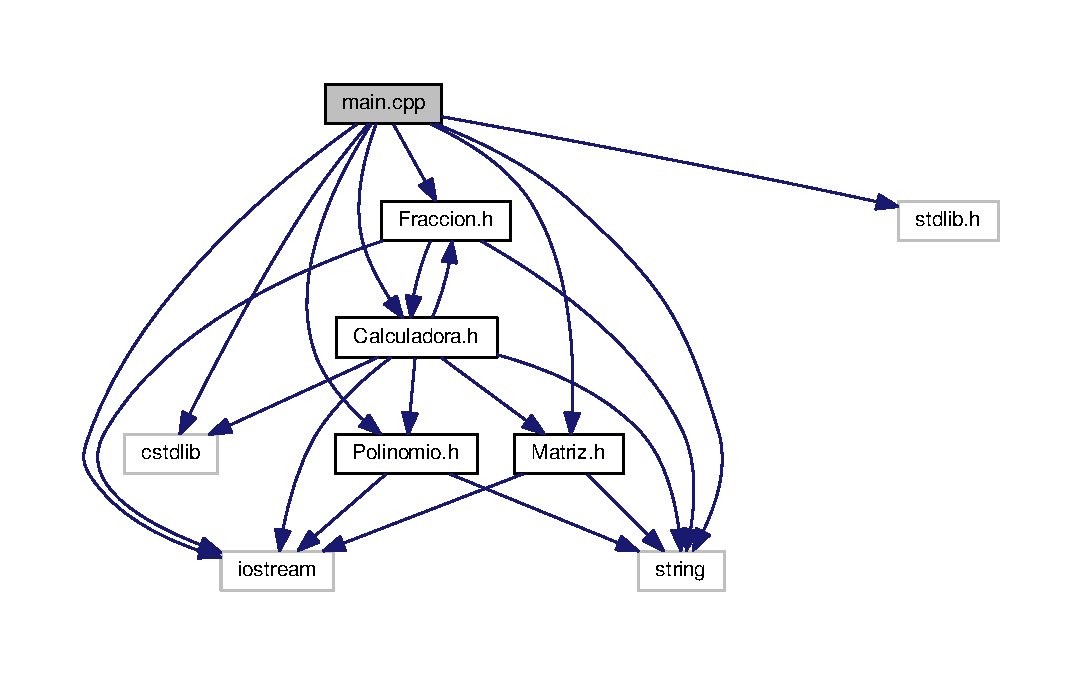
\includegraphics[width=350pt]{main_8cpp__incl}
\end{center}
\end{figure}
\subsection*{Macros}
\begin{DoxyCompactItemize}
\item 
\#define \hyperlink{main_8cpp_a4fc34b120ed3bd1120c1eb36abbcd6af}{N\+L}~cout $<$$<$ endl;
\item 
\#define \hyperlink{main_8cpp_aecd69d9a67487cc45c38eb184c50538a}{S\+P}~\char`\"{} \char`\"{}
\end{DoxyCompactItemize}
\subsection*{Functions}
\begin{DoxyCompactItemize}
\item 
int \hyperlink{main_8cpp_a3c04138a5bfe5d72780bb7e82a18e627}{main} (int argc, char $\ast$$\ast$argv)
\end{DoxyCompactItemize}


\subsection{Macro Definition Documentation}
\hypertarget{main_8cpp_a4fc34b120ed3bd1120c1eb36abbcd6af}{\index{main.\+cpp@{main.\+cpp}!N\+L@{N\+L}}
\index{N\+L@{N\+L}!main.\+cpp@{main.\+cpp}}
\subsubsection[{N\+L}]{\setlength{\rightskip}{0pt plus 5cm}\#define N\+L~cout $<$$<$ endl;}}\label{main_8cpp_a4fc34b120ed3bd1120c1eb36abbcd6af}
\hypertarget{main_8cpp_aecd69d9a67487cc45c38eb184c50538a}{\index{main.\+cpp@{main.\+cpp}!S\+P@{S\+P}}
\index{S\+P@{S\+P}!main.\+cpp@{main.\+cpp}}
\subsubsection[{S\+P}]{\setlength{\rightskip}{0pt plus 5cm}\#define S\+P~\char`\"{} \char`\"{}}}\label{main_8cpp_aecd69d9a67487cc45c38eb184c50538a}


\subsection{Function Documentation}
\hypertarget{main_8cpp_a3c04138a5bfe5d72780bb7e82a18e627}{\index{main.\+cpp@{main.\+cpp}!main@{main}}
\index{main@{main}!main.\+cpp@{main.\+cpp}}
\subsubsection[{main}]{\setlength{\rightskip}{0pt plus 5cm}int main (
\begin{DoxyParamCaption}
\item[{int}]{argc, }
\item[{char $\ast$$\ast$}]{argv}
\end{DoxyParamCaption}
)}}\label{main_8cpp_a3c04138a5bfe5d72780bb7e82a18e627}


Here is the call graph for this function\+:\nopagebreak
\begin{figure}[H]
\begin{center}
\leavevmode
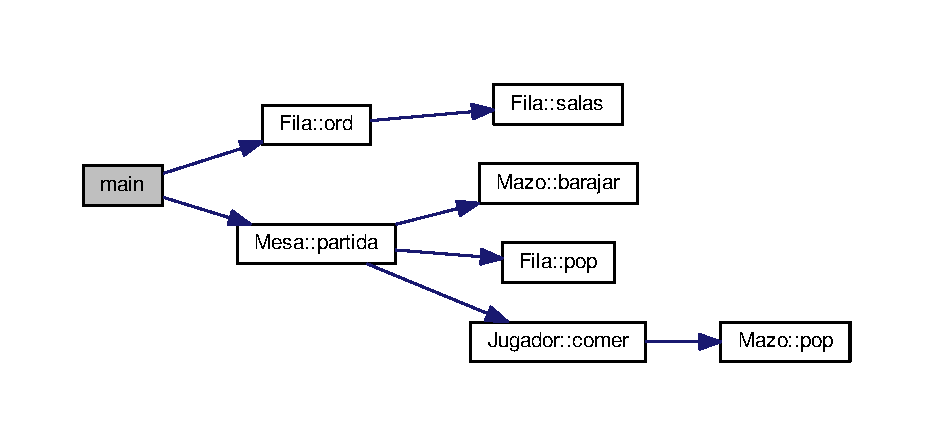
\includegraphics[width=240pt]{main_8cpp_a3c04138a5bfe5d72780bb7e82a18e627_cgraph}
\end{center}
\end{figure}



\hypertarget{_matriz_8cpp}{\section{code/\+Matriz.cpp File Reference}
\label{_matriz_8cpp}\index{code/\+Matriz.\+cpp@{code/\+Matriz.\+cpp}}
}
{\ttfamily \#include \char`\"{}Matriz.\+h\char`\"{}}\\*

\hypertarget{_matriz_8h}{\section{code/\+Matriz.h File Reference}
\label{_matriz_8h}\index{code/\+Matriz.\+h@{code/\+Matriz.\+h}}
}
{\ttfamily \#include $<$cstdlib$>$}\\*
{\ttfamily \#include $<$iostream$>$}\\*
{\ttfamily \#include \char`\"{}string\char`\"{}}\\*
\subsection*{Classes}
\begin{DoxyCompactItemize}
\item 
class \hyperlink{class_matriz}{Matriz}
\end{DoxyCompactItemize}

\hypertarget{_polinomio_8cpp}{\section{Polinomio.\+cpp File Reference}
\label{_polinomio_8cpp}\index{Polinomio.\+cpp@{Polinomio.\+cpp}}
}
{\ttfamily \#include \char`\"{}Polinomio.\+h\char`\"{}}\\*
Include dependency graph for Polinomio.\+cpp\+:
\nopagebreak
\begin{figure}[H]
\begin{center}
\leavevmode
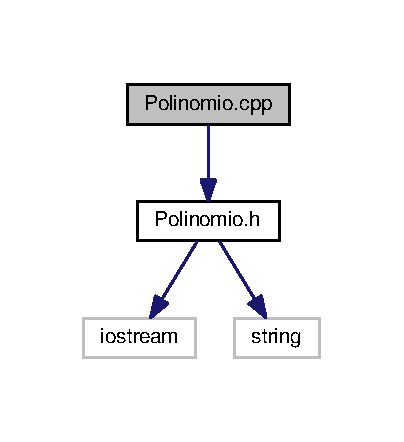
\includegraphics[width=194pt]{_polinomio_8cpp__incl}
\end{center}
\end{figure}

\hypertarget{_polinomio_8h}{\section{code/\+Polinomio.h File Reference}
\label{_polinomio_8h}\index{code/\+Polinomio.\+h@{code/\+Polinomio.\+h}}
}
{\ttfamily \#include $<$iostream$>$}\\*
{\ttfamily \#include \char`\"{}string\char`\"{}}\\*
\subsection*{Classes}
\begin{DoxyCompactItemize}
\item 
class \hyperlink{class_polinomio}{Polinomio}
\end{DoxyCompactItemize}

%--- End generated contents ---

% Index
\newpage
\phantomsection
\addcontentsline{toc}{chapter}{Index}
\printindex

\end{document}
